\RequirePackage{xcolor}
\documentclass[a0]{sciposter} % mayor hoja estandar
\usepackage{multicol,subfig,amsmath}
\usepackage{graphicx,url,hyperref,doi}
\usepackage[spanish]{babel}   
\usepackage[utf8]{inputenc}
\usepackage[sort&compress,numbers]{natbib}
\usepackage{tikz}

\tikzstyle{elem} = [draw, rectangle, thick, minimum height=2em, minimum width=2em]
\tikzstyle{line} = [draw, thick, -stealth, shorten >=1pt]

\setlength{\parskip}{1.5pt}
\renewcommand{\arraystretch}{1.5}

\title{Relación entre el número de ingresos hospitalarios y los niveles de contaminación}
\author{Abraham Zaragoza$^\dagger$, Selene Prado$^\ddagger$ y Elisa Schaeffer$^\ast$}
\institute {Ingeniería en Tecnología de Software $^\dagger$$^\ddagger$, Posgrado en Ingeniería de Sistemas $^\ast$}
\email{abraham.zaragozagrc@uanl.edu.mx $^\dagger$, selene.pradopr@uanl.edu.mx $^\ddagger$, elisa.schaeffer@uanl.edu.mx $^\ast$}
\leftlogo[1]{uanl.png} 
\rightlogo[1]{fime.png}

\begin{document}

% QR y nuevo logo
\conference{\raisebox{2cm}[0cm]{
\includegraphics[width=80mm]{paicyt2021.png}}
  \hfill
  \raisebox{2cm}[0cm]{
\includegraphics[width=40mm]{qr-code.png}}
  \hfill
  \raisebox{2cm}[0cm]{
\includegraphics[width=100mm]{verano.png}}}

\maketitle

\begin{multicols}{2} 

\begin{abstract}
Se presenta una función codificada en Python 3.9 \citep{python} que realiza gráficos de telaraña de determinado conjunto de datos. Como entrada se tienen datos de la Secretaría de Salud del Gobierno de México y registros de los niveles de los contaminantes presentes en el área metropolitana de Monterrey. Con ello se obtienen gráficos de radar para mostrar visualmente el número de ingresos hospitalarios y los niveles de NO2, NOX, PM10, y PM2.5 durante los años 2015, 2016, 2017, y 2018.
\end{abstract}

\section{Introducción}

Se tienen los datos de ingresos hospitalarios desde el año 2015 hasta el año 2018, los cuales provienen de la base de datos de la Secretaría de Salud del Gobierno de México. También se tienen los registros de los niveles de los contaminantes NO2, NOX, PM10, y PM2.5 presentes en el área metropolitana de Monterrey de los años mencionados anteriormente, dichos registros son hechos por las estaciones: Sureste, Noreste, Centro, Noroeste, Suroeste, Noroeste2, Noreste2, Norte, Sureste2, Suroeste2, Sureste3, Norte2, y Sur.
Se tiene la hipótesis de que el número de de ingresos hospitalarios aumenta cuando los niveles de contaminación del aire incrementan. 
El objetivo del presente proyecto es fomentar la regulación del nivel de contaminantes emitidos en el área metropolitana de Monterrey, así como explorar potenciales relaciones entre el aumento del nivel de contaminantes y la salud pública.

\section{Antecedentes}

Algunos conceptos importantes a definir para este proyecto son:  
\begin{itemize}
    \item Contaminación atmósferica: \citet{bib4} mencionan que la contaminación atmósferica es la presencia de materia o formas de energía en el aire que impliquen algún daño para las personas.
    \item Ingreso hospitalario: Un ingreso hospitalario involucra una serie de actividades técnico administrativo que se llevan a cabo en los centros de salud para ingresar a un paciente.
    \item Salud: En \citet{bib3} se define la salud como un completo estado de bienestar tanto físico como mental y social.
    \item Gráfico de radar: También conocido como diagrama de araña, es un método gráfico para mostrar datos multivariados en forma de un gráfico bidimensional de tres o más variables cuantitativas representadas en ejes que comienzan desde el mismo punto (\citet{bib5}).  
\end{itemize}
 Los contaminantes estudiados en el presente trabajo son: dióxido de nitrógeno (NO2), óxidos de nitrógeno (NOX), partículas PM10, y partículas PM2.5.

%\columnbreak

\section{Estado de arte}

\citet{bib1} señala la deficiencia en las acciones del gobierno ante la contaminación del aire y como se ve reducido a reportar los niveles de toxicidad, asi como recomendar acciones en caso de contingencia ambiental. Haciendo uso de los datos del Comité Estatal de Vigilancia Epidemiologica del estado de Jalisco, asi como los datos obtenidos por el Sistema de Monitoreo Atmosférico de Jalisco, se obtiene una correlación significativa para los contaminantes como el monoxido de carbono y particulas menores a 10 micras, las cuales infieren en mayor manera a las Infecciones Respiratorias Agudas. 

\section{Solución propuesta}

Se tiene la función create\_spiderwebs que crea gráficos de radar a partir de conjuntos de datos. 
La implementación está hecha en Python 3.9 \citep{python}. Se puede acceder al repositorio del presente trabajo mediante el código QR que se encuentra en la parte inferior, en dicho repositorio se encuentra el programa mencionado anteriormente. Los parametros que recibe dicha función se explican en el cuadro \ref{fparametros}. 

\begin{table}
\setcounter{table}{0} % por culpa de sciposter
\captionsetup{type=table} % por culpa de sciposter
\caption{Párametros de la función create\_spiderwebs.}
\label{fparametros}
\begin{center}
\scalebox{0.8}{\begin{tabular}{|l|l|}
    \hline
         \multicolumn{1}{|l|}{{\bf Parámetro}}
         & \multicolumn{1}{|l|}{{\bf Descripción\phantom{m}}} \\
         \hline
         datasets & Lista que contiene una lista por cada conjunto de datos \\
         \hline
         lenlines & Número entero que representa la longitud de cada línea en los gráficos de telaraña \\
        \hline
        numspiders & Número de gráficos de telaraña a generar \\
        \hline
        title & Título de la figura \\
        \hline
        titles & Lista con los nombres de cada gráfico en la figura \\
        \hline
        spoke\_labels & Lista con los nombres de cada línea en el gráfico \\
        \hline
        colors & Lista con la primera letra del color de cada gráfico \\ 
        & ('b' = azul, 'r' = rojo, 'g' = verde, 'm' = magenta, 'y' = amarillo) \\
        \hline
        typeframe & Nombre del tipo de marco para el gráfico ('circle' o 'polygon') \\
        \hline
    \end{tabular}}
\end{center}
\end{table}

Para el tratamiento de los datos y el uso de la función se utiliza Jupyter Notebook \citep{jupyter}. Las libretas se encuentran en el repositorio del presente trabajo.

\section{Experimentos}

Se tienen gráficas de radar de los niveles de los contaminantes de NO2, NOX, PM10, y PM2.5 durante las primeras 6 semanas de los años 2015, 2016, 2017, y 2018, dichas figuras se encuentran en el repositorio. En la figura \ref{contaminantes} se muestran los gráficos obtenidos de los años 2015 y 2017. 

\begin{figure}
\setcounter{figure}{0} % por culpa de sciposter
\captionsetup{type=figure} % por culpa de sciposter
\begin{center}
   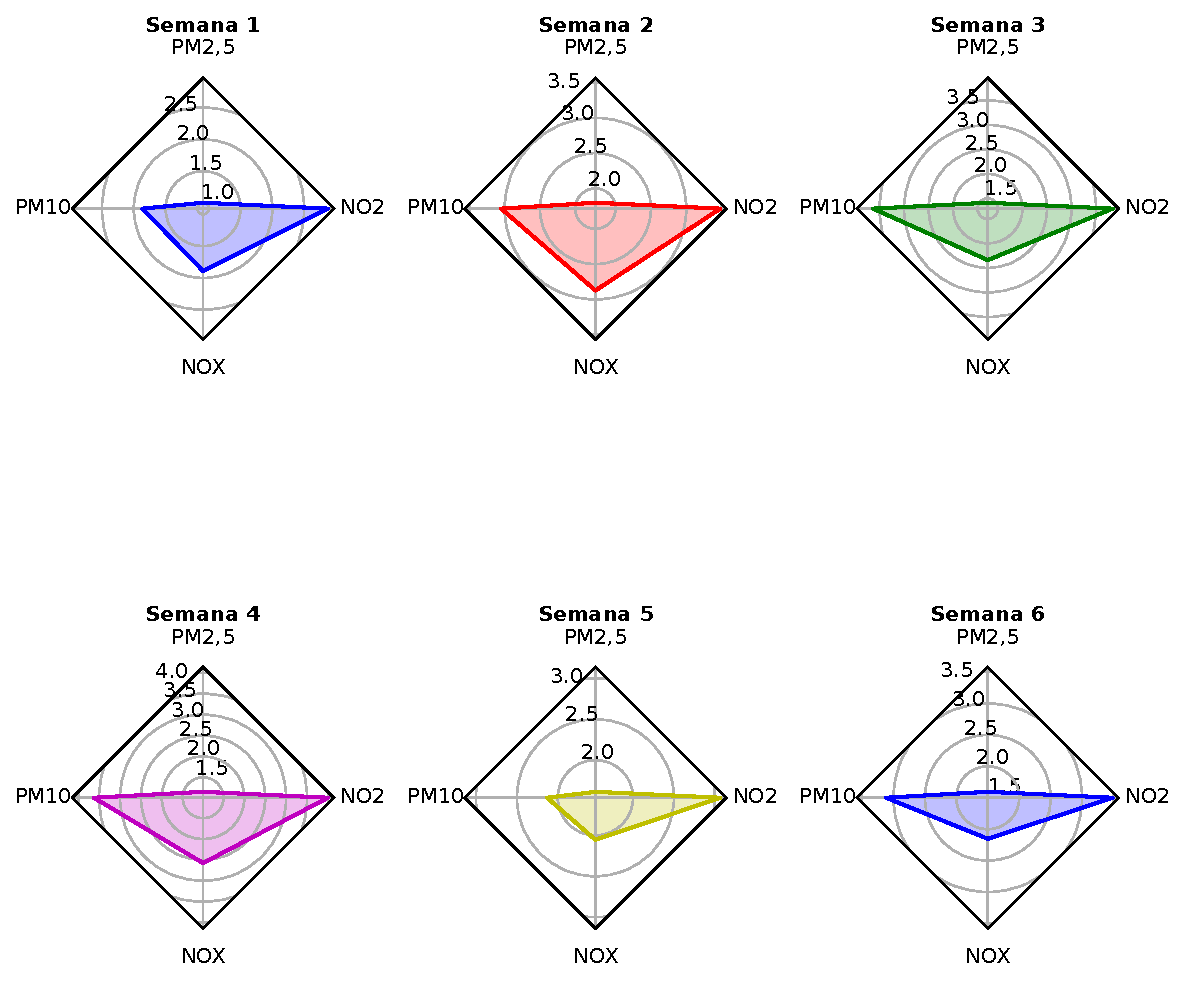
\includegraphics[width=0.4\textwidth]{Contaminantes-2015.eps}
   \hspace{2cm}
   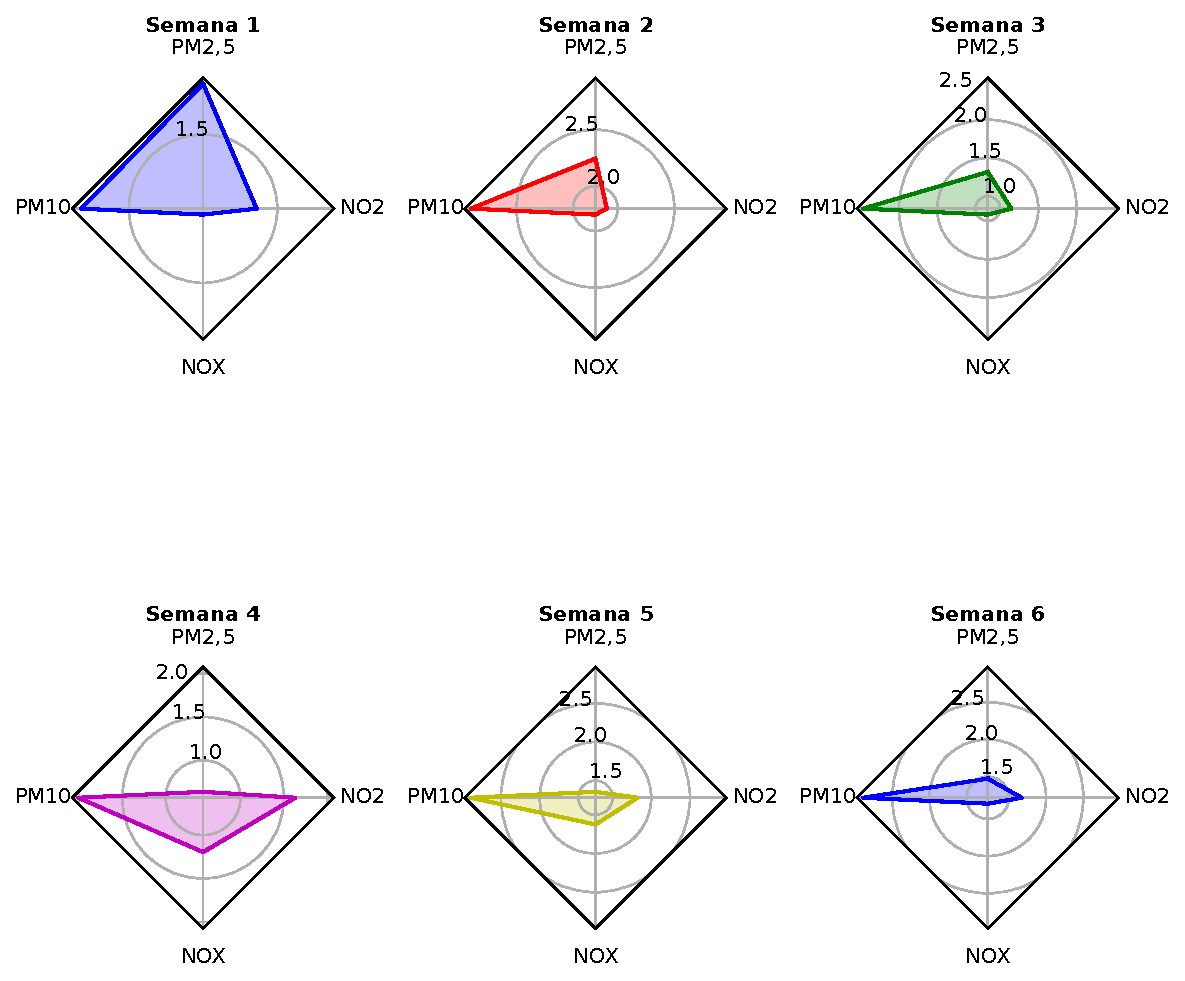
\includegraphics[width=0.4\textwidth]{Contaminantes-2017.eps}
   \end{center}
    \caption{Niveles de los contaminantes NO2, NOX, PM10 y PM2.5 durante las primeras 6 semanas de los años 2015 y 2017.}
    \label{contaminantes}
\end{figure}

La figura \ref{ingresos} muestra el número de ingresos hospitalarios durante las primeras 6 semanas de los años 2015, 2016, 2017, y 2018.

\begin{figure}
\setcounter{figure}{1} % por culpa de sciposter
\captionsetup{type=figure} % por culpa de sciposter
\begin{center}
   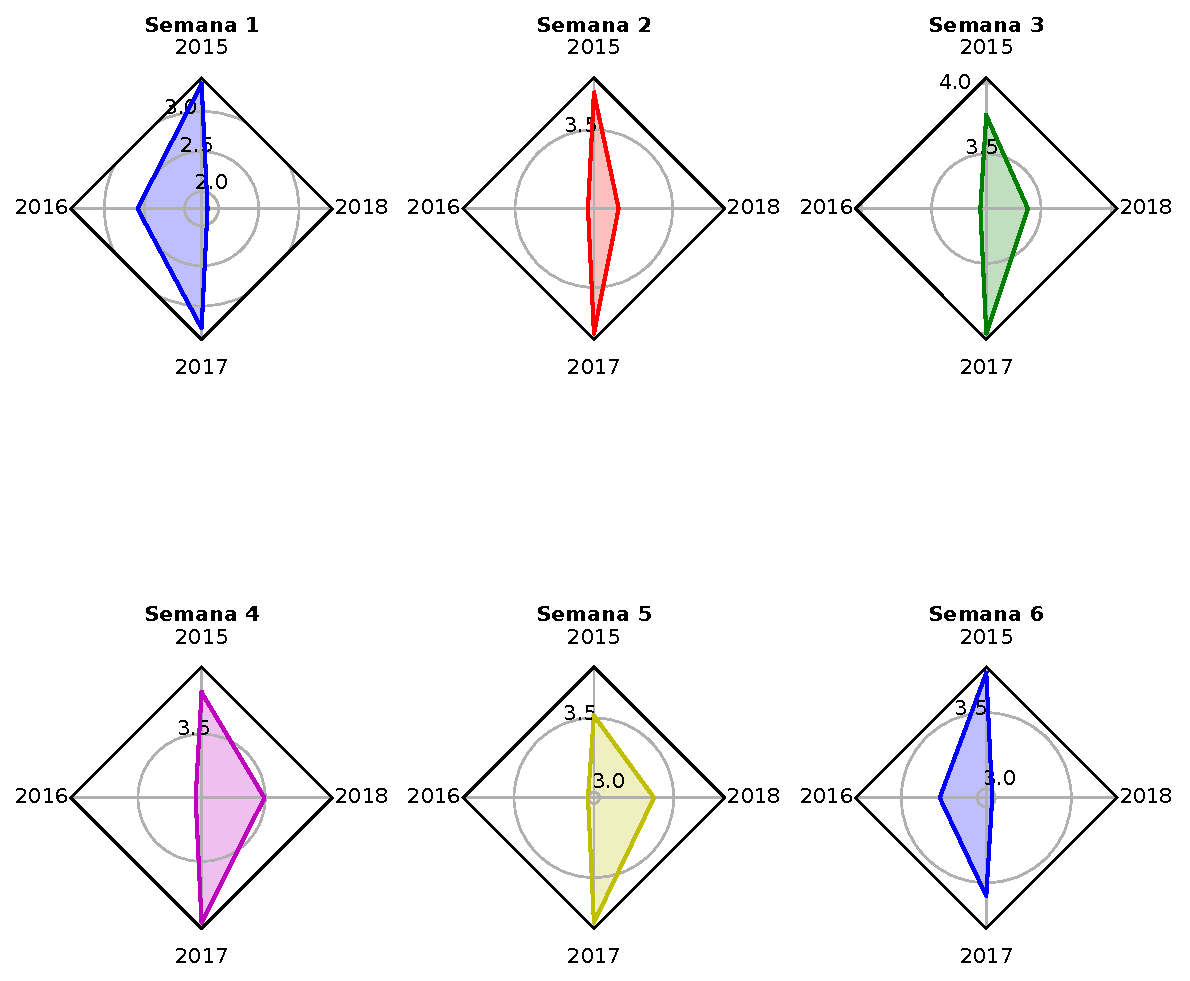
\includegraphics[width=0.4\textwidth]{Ingresos-hospitalarios.eps}
   \end{center}
    \caption{Número de ingresos hospitalarios en las primeras 6 semanas de los años 2015, 2016, 2017, y 2018.}
    \label{ingresos}
\end{figure}


\section{Conclusiones}
Se encontró que durante durante las primeras 6 semanas de los años 2015 y 2016 el nivel de NO2 se mantuvo más alto que los otros 3 contaminantes. En el año 2017 se encontró que fue el PM10 el que se mantuvo más alto, y en el 2018 fue el PM2.5. Así mismo se pudo ver que los años 2015 y 2017 fueron los años que más ingresos hospitalarios presentaron durante las primeras 6 semanas del año. 
Con lo anterior se puede concluir que puede haber una relación entre el aumento de los niveles de NO2 y PM10 y el aumento de ingresos hospitalarios.
En un próximo trabajo se pueden realizar gráficas de más semanas y extraer de las bases de datos que se tiene los ingresos hospitalarios por infecciones respiratorias.

\subsection*{Agradecimientos}

Se cuenta con el financiamiento del programa PAICYT-UANL bajo las claves CE1421-20 y CE1842-21.\\
El póster se preparó con \url{https://www.overleaf.com/}.

\bibliography{poster}
\bibliographystyle{plainnat}
    
\end{multicols}

\end{document}
